\documentclass{article}
\usepackage{geometry}
\geometry{a4paper, left=1.5in, bottom=1in, right=1.5in, top=1in}
\usepackage{color}
\usepackage{hyperref}
\usepackage{amsmath}
\usepackage{multirow}
\usepackage{pdflscape}
\usepackage[table]{xcolor}
\usepackage{hhline}
\usepackage{graphicx}
%%%%%%%%%%%%%%%%%%%%%%%%%%%%%%%%%%%%%%%%%%%%%%%%%%%
%%%%%%%%%%%%%%% end of preamble %%%%%%%%%%%%%%%%%
%%%%%%%%%%%%%%%%%%%%%%%%%%%%%%%%%%%%%%%%%%%%%%%%%%%%%%%



%%%%%%%%%%%%%%%%%%%%%%%%%%%%%%%%%%%%%%%%%%%%%%%%
%%%%%%%%%%%%%%%%% begin document %%%%%%%%%%%%%%%%%%
%%%%%%%%%%%%%%%%%%%%%%%%%%%%%%%%%%%%%%%%%%%%%%%%%%%%%
\begin{document}
%%%%%%%%%%%%%%%%%%%%%%%%%%%%%%%%%%%%%%%%%%%%%%%%%%%%%%
%%%%%%%%%%%%%%%% titles% %%%%%%%%%%%%%%%%%%%%%%%%%%%%%5
%%%%%%%%%%%%%%%%%%%%%%%%%%%%%%%%%%%%%%%%%%%%%%%%%%%%%%%%%
\title{Image Quality for Deep Learning}
\author{Pooryaa Cheraaqee}
\maketitle


%%%%%%%%%%%%%%%%%%%%%%%%%%%%%%%%%%%%%%%%%%%%%
%%%%%%%%%%%% begin Introduction %%%%%%%%%%%%%%%%
%%%%%%%%%%%%%%%%%%%%%%%%%%%%%%%%%%%%%%%%%%%%%%
\section{Introduction} \label{sec:introductoin}
Digitized images are a prevalent medium in the Internet communications and a large portion of our information are conveyed by images and visual signals~\cite{cisco}. It is apparent that the unpleasant quality of such media can prevent us from obtaining the information that we desire or may cause disturbing viewing experiences. The same thing is possible to happen for the machines. To be clear, artificial intelligence (AI) algorithms use images as training data and if the quality of the data that is fed to such machine learning algorithms is poor, the algorithm may deviate from its normal performance.

Convolutinal neural networks (CNNs) are at the heart of a large number of computer vision applications, such as license plate recognition, face recognition, image classification, and object detection~\cite{goodfellow2016deep}. These networks operate by training on a set of images (dataset) and applying the gained knowledge in their task. Since CNNs are vitial for automating many tedious tasks, it is important to assure that the data which they are training on, is of adequate quality. One way to acheive this, is comming up with an objective measure of image quality that represents how well the CNN will perform if it is fed with this image for training or inference. Having such method for quantifying the quality of images for machine perception, we can automatically optimize deep learning datasets or discard missinformative image samples.

Image quality has been investigated by researchers and practitioners since the early days of photograpy~\cite{allen2012manual}. Human has usually been considered as the ultimate viewer of images and hence the most reliable measures of quality were provided by \emph{subjective} assessments~\cite{chandler2013seven}. During a subjective image quality assessment (IQA), a statistically sufficient number of observers (subjects) view an image and give a score to its quality (either as a number in the $[0, 10]$ interval or with any other psychometric scales~\cite{stevens1946theory}). Their mean opinion score (MOS\footnote{MOS is in a direct proportion with the perceived quality and \emph{difference}-MOS (DMOS) is in inverse proportion with the perceived quality. To make it convinient, we can state that MOS measures quality and DMOS measures \emph{distotion} or artefact's severity.}) provides a quantification of image quality. Due to the inconvinience of subjective experiments for on-line and large-scale applications, computational models are desired that can predict human judgements on image quality. The results of subjective experiments are used as a ground-truth for validating and training objective models~\cite{seshadrinathan2011automatic}. 

As mentioned, the IQA research has been mostly concerned with human satisfaction of images, while it has been shown that metrifying image quality for other objectives is quite different~\cite{ye2013document}. In particular, to see how image quality can affect the performance deep neural networks, we need a model, $f$. $f$ inputs an image, $I$, and produces a \textbf{bounded} value, such as in $[0, 1]$. That is, $f(I) \in [0, 1]$, and $f(I)$ correlates with the performance of CNN in learning from $I$ or making inferences about $I$. It is also desired that the model can point out the flaws or distortions that have possibly made $I$ inappropriate for using in a deep learning pipeline.

Apart from physically measuring image attributes or quality dimensions and devising explicit features, the problem can be tackled in an end-to-end paradigm. After presenting a background, a potential solution will be formulated in the section~\ref{sec:proposed_method}.
%%%%%%%%%%%%%%%%%%%%%%%%%%%%%%%%%%%%%%%%%%%%%%%%%%%%%%%%%%%%%
%%%%%%%%%%%%%%%%%%%%%%% end Introduction %%%%%%%%%%%%%%%%%%%%
%%%%%%%%%%%%%%%%%%%%%%%%%%%%%%%%%%%%%%%%%%%%%%%%%%%%%%%%5%%%

%%%%%%%%%%%%%%%%%%%%%%%%%%%%%%%%%%%%%%%%%%%%%%%%%%%%%%
%%%%%%%%%%%%%%%%%%%%% begin Background %%%%%%%%%%%%%%%%%
%%%%%%%%%%%%%%%%%%%%%%%%%%%%%%%%%%%%%%%%%%%%%%%%%%%%%%%%%%5
\section{Background} \label{background}
The most common researches for quality assessment (QA) of digitized images has recently belonged to the category of \emph{computational metrics} as classified by Fry et. al.~\cite{fry2018bridging}. These methods are validated with subjective experiments~\cite{zhai2020perceptual}. These subjective experiments are published as datasets which are essentially sets of $(image, MOS/DMOS)$ ordered pairs. An objective method is applied to the images and its output is expected to correlate with the MOS/DMOS of images in the dataset. (The correlation is expressed with common correlation indices, such as Pearson linear correlation index (PLCC) and Spearman rank order correlation index (SROCC).)

A classification of IQA methods based on the availability of a pristine signal is good to be made here. In some applications, such as image compression, there are two images available: the initial raw image and the compressed image that may suffer from blocking or ringing artefacts. Suppose the lossy compression algorithm embeds a quality metric to assess the compressed image and in the case of a dire quality, automatically regulates its loss parameters. This quality metric has the pristine image in addition to the test image at its disposal and can use it as a reference. This is an example of \emph{full-reference} (FR) IQA. In communcation settings, where the pristine signals are bulky to transmit, certain features can be extracted and sent over to aid the assessment of a distorted image (\emph{reduced-reference} (RR) IQA). \emph{No-reference} (NR) IQA is the case that the quality of an image is to be assessed without any information of its pristine version. (If such a reference even exists, like what happens in a DSLR camera.) It is believed that NR IQA is more difficult than the other cases~\cite{kang2014convolutional}.

Early FR computational metrics were based on error visibility. If $ref(x, y)$ and $dst(x, y)$ are the luminance components of the reference and the distorted images and they are both of dimensions $M\times N$, the mean squared error (MSE) for them is defined as:
\begin{equation}
	\label{eq:mse}
	\displaystyle MSE(ref, dst) = \frac{1}{M\times N}\sum_{x=1}^M \sum_{y = 1}^N \left(ref(x, y)-dst(x, y)\right)^2
\end{equation}
Peak signal to noise ratio (PSNR) is also based on MSE. It has been shown that these methods do not necessarily correlate with human perception of quality~\cite{wang2009mean}.

Wang et. al.~\cite{wang2002universal} showed that structures can be a reasonable criterion for image quality and proposed a method to metrify structural similarity (SSIM) in 2004~\cite{wang2004image}. With the success of SSIM, other methods tried to express structures with other features, such as image edges~\cite{chen2006edge} and gradients~\cite{Xue2014}. Natural scene statistics~\cite{moorthy2011blind} and information fidelity~\cite{sheikh2006image} are other criteria for image quality. End-to-end machine learning is also exploited for the task of objective IQA~\cite{yang2019survey, ye2012unsupervised,kim2017deep}.

Document image quality assessment (DIQA) is an example of measuring quality for an objective other than human perception~\cite{ye2013document}. The ground-truth for DIQA methods is not human opinion, but the accuracy of optical character recognition (OCR) methods. The DIQA metric needs to predict how accurate an OCR method will perform on the given image. The same approach can be taken for evaluating an image's suitability for deep learning tasks. A similar problem is video coding for machine~\cite{duan2020video}, where the goal is to optimize the coding with the assumption that an algorithm is going consume the uncompressed data for some recognition task.
%%%%%%%%%%%%%%%%%%%%%%%%%%%%%%%%%%%%%%%%%%%%%%%%%%%%%%%%%%%
%%%%%%%%%%%%%%%%%%%%%%% end Background %%%%%%%%%%%%%%%%%%
%%%%%%%%%%%%%%%%%%%%%%%%%%%%%%%%%%%%%%%%%%%%%%%%%%%%%%%%%%%%


%%%%%%%%%%%%%%%%%%%%%%%%%%%%%%%%%%%%%%%%%%%%%%%%%%%%%%%%%%%%
%%%%%%%%%%%%%%%% begin Proposed Method %%%%%%%%%%%%%%%%%%
%%%%%%%%%%%%%%%%%%%%%%%%%%%%%%%%%%%%%%%%%%%%%%%%%%%%%%%%%%%
\section{Proposed Method} \label{sec:proposed_method}
Convolutional neural networks can be considered as a function that maps an image to some output. This output can be a number, multiple numbers, another image, a label, a combination of numbers and labels, etc. No matter what is the output, the network needs a ground-truth to guide it in tuning its weights. If $x$ is the input image, then $y = CNN(x)$ is the output of the network and $\hat{y}$ is the correct answer for $x$. Some measure of error (\emph{loss function}) tells the network how bad $y$ is; according to $\hat{y}$: $\text{error}_x=loss(y, \hat{y})$. The network then tries to minimize the $\text{error}$ with each labeled sample that it is fed with.

We need a model, $f$, that given $x$, predicts network's error for $x$. That is, ideally:
\begin{equation}
	\label{eq:model}
	f(x) = \text{error}_x, x\in D
\end{equation}
\subsection{End-to-End Approach} \label{sec:end_to_end}
Given a labeled dataset, $D$, for a CNN task, the network can be applied to each sample and an error can be computed accordingly. Each image, $x$, in $D$ can be distorted using synthesized artefacts, such as Gaussian blur, Gaussian noise, and JPEG compression as in image quality datasets~\cite{sheikh2005live}. Each artefact, $a$, can be applied at various levels of severity, $l$. It is hoped that the network performance, $error$, has a meaningful relation with $l$.

The ground-truth for $x$ in $D$ is represented as $\hat{y}_x$. It is clear that the distorted version of $x$ with artifcat $a$ at level $l$, $x_{a, l}$, will have the same ground-truth for the task of $D$. To compute the error of the CNN for each $x_{a,l}$, the same $\hat{y}_x$ can be used: $\text{error}_{x_{a, l}} = loss(CNN(x_{a,l}), \hat{y}_x), a\in A, l\in L$, where $A$ is the set of all distortion types employed and $L$ is the set of all levels of severity.

By computing $\text{error}_{x_{a, l}}$ for all combinations of $x$s, $a$s, and $l$s, we will have a set of ordered pairs like $(x_{a, l}, error_{x_{a, l}})$. This set, $D\prime$, can serve as a dataset for training a second CNN, called $CNN_{metrifier}$. $CNN_{metrifier}$ receives an image and tries to learn what error the $CNN$ will make on this image. A sucessful $CNN_{metrifier}$ can serve as the model $f$ in~(\ref{eq:model}).
\subsection{Bottom-up Approach} \label{sec:bottom_up}
Characteristics of human visual system (HVS) have been discovered, modeled, and employed in predicting our judgements of image quality~\cite{zhai2020perceptual, fry2018bridging}. CNNs can be analogous to HVS and trying to interpret their inner-mechanism may reveal some traits that can be explicitly used to measure image dimensions and their effect on network performance. A probable phenomenon to witness is that the effect of distortions may be more apparent in the early layers of a network in comparison to the ending layers that are more semantic. The network architectural characteristics, such as drop-out layers, can also have alleviating effects in propagating the distortions.

It is worth to note that the approach proposed in section~\ref{sec:end_to_end} was task agnostic. However, it is probably different to predict the performance of an image classifier on an image than an object detector. A more detailed formulation of the proposed method may be found in the Jupyter notebooks at \href{https://github.com/cheraaqee/iqa\_for\_cnn}{https://github.com/cheraaqee/iqa\_for\_cnn}.
%%%%%%%%%%%%%%%%%%%%%%%%%%%%%%%%%%%%%%%%%%%%%%%%%%%%%%%%
%%%%%%%%%%%%%%%%%%%%% end Proposed Method %%%%%%%%%%%%%%%
%%%%%%%%%%%%%%%%%%%%%%%%%%%%%%%%%%%%%%%%%%%%%%%%%%%%%%%%

%%%%%%%%%%%%%%%%%%%%%%%%%%%%%%%%%%%%%%%%%%%%%%%%%%%%%%%%
%%%%%%%%%%%%%%%%%%%% begin Timing & Plan %%%%%%%%%%%%%%%
%%%%%%%%%%%%%%%%%%%%%%%%%%%%%%%%%%%%%%%%%%%%%%%%%%%%%%%
\section{Timing\& Plan} \label{sec:timing_plan}
Figure~\ref{fig:gantt} provides an overview of the tasks considered for the research.
\begin{landscape}
\begin{figure}
	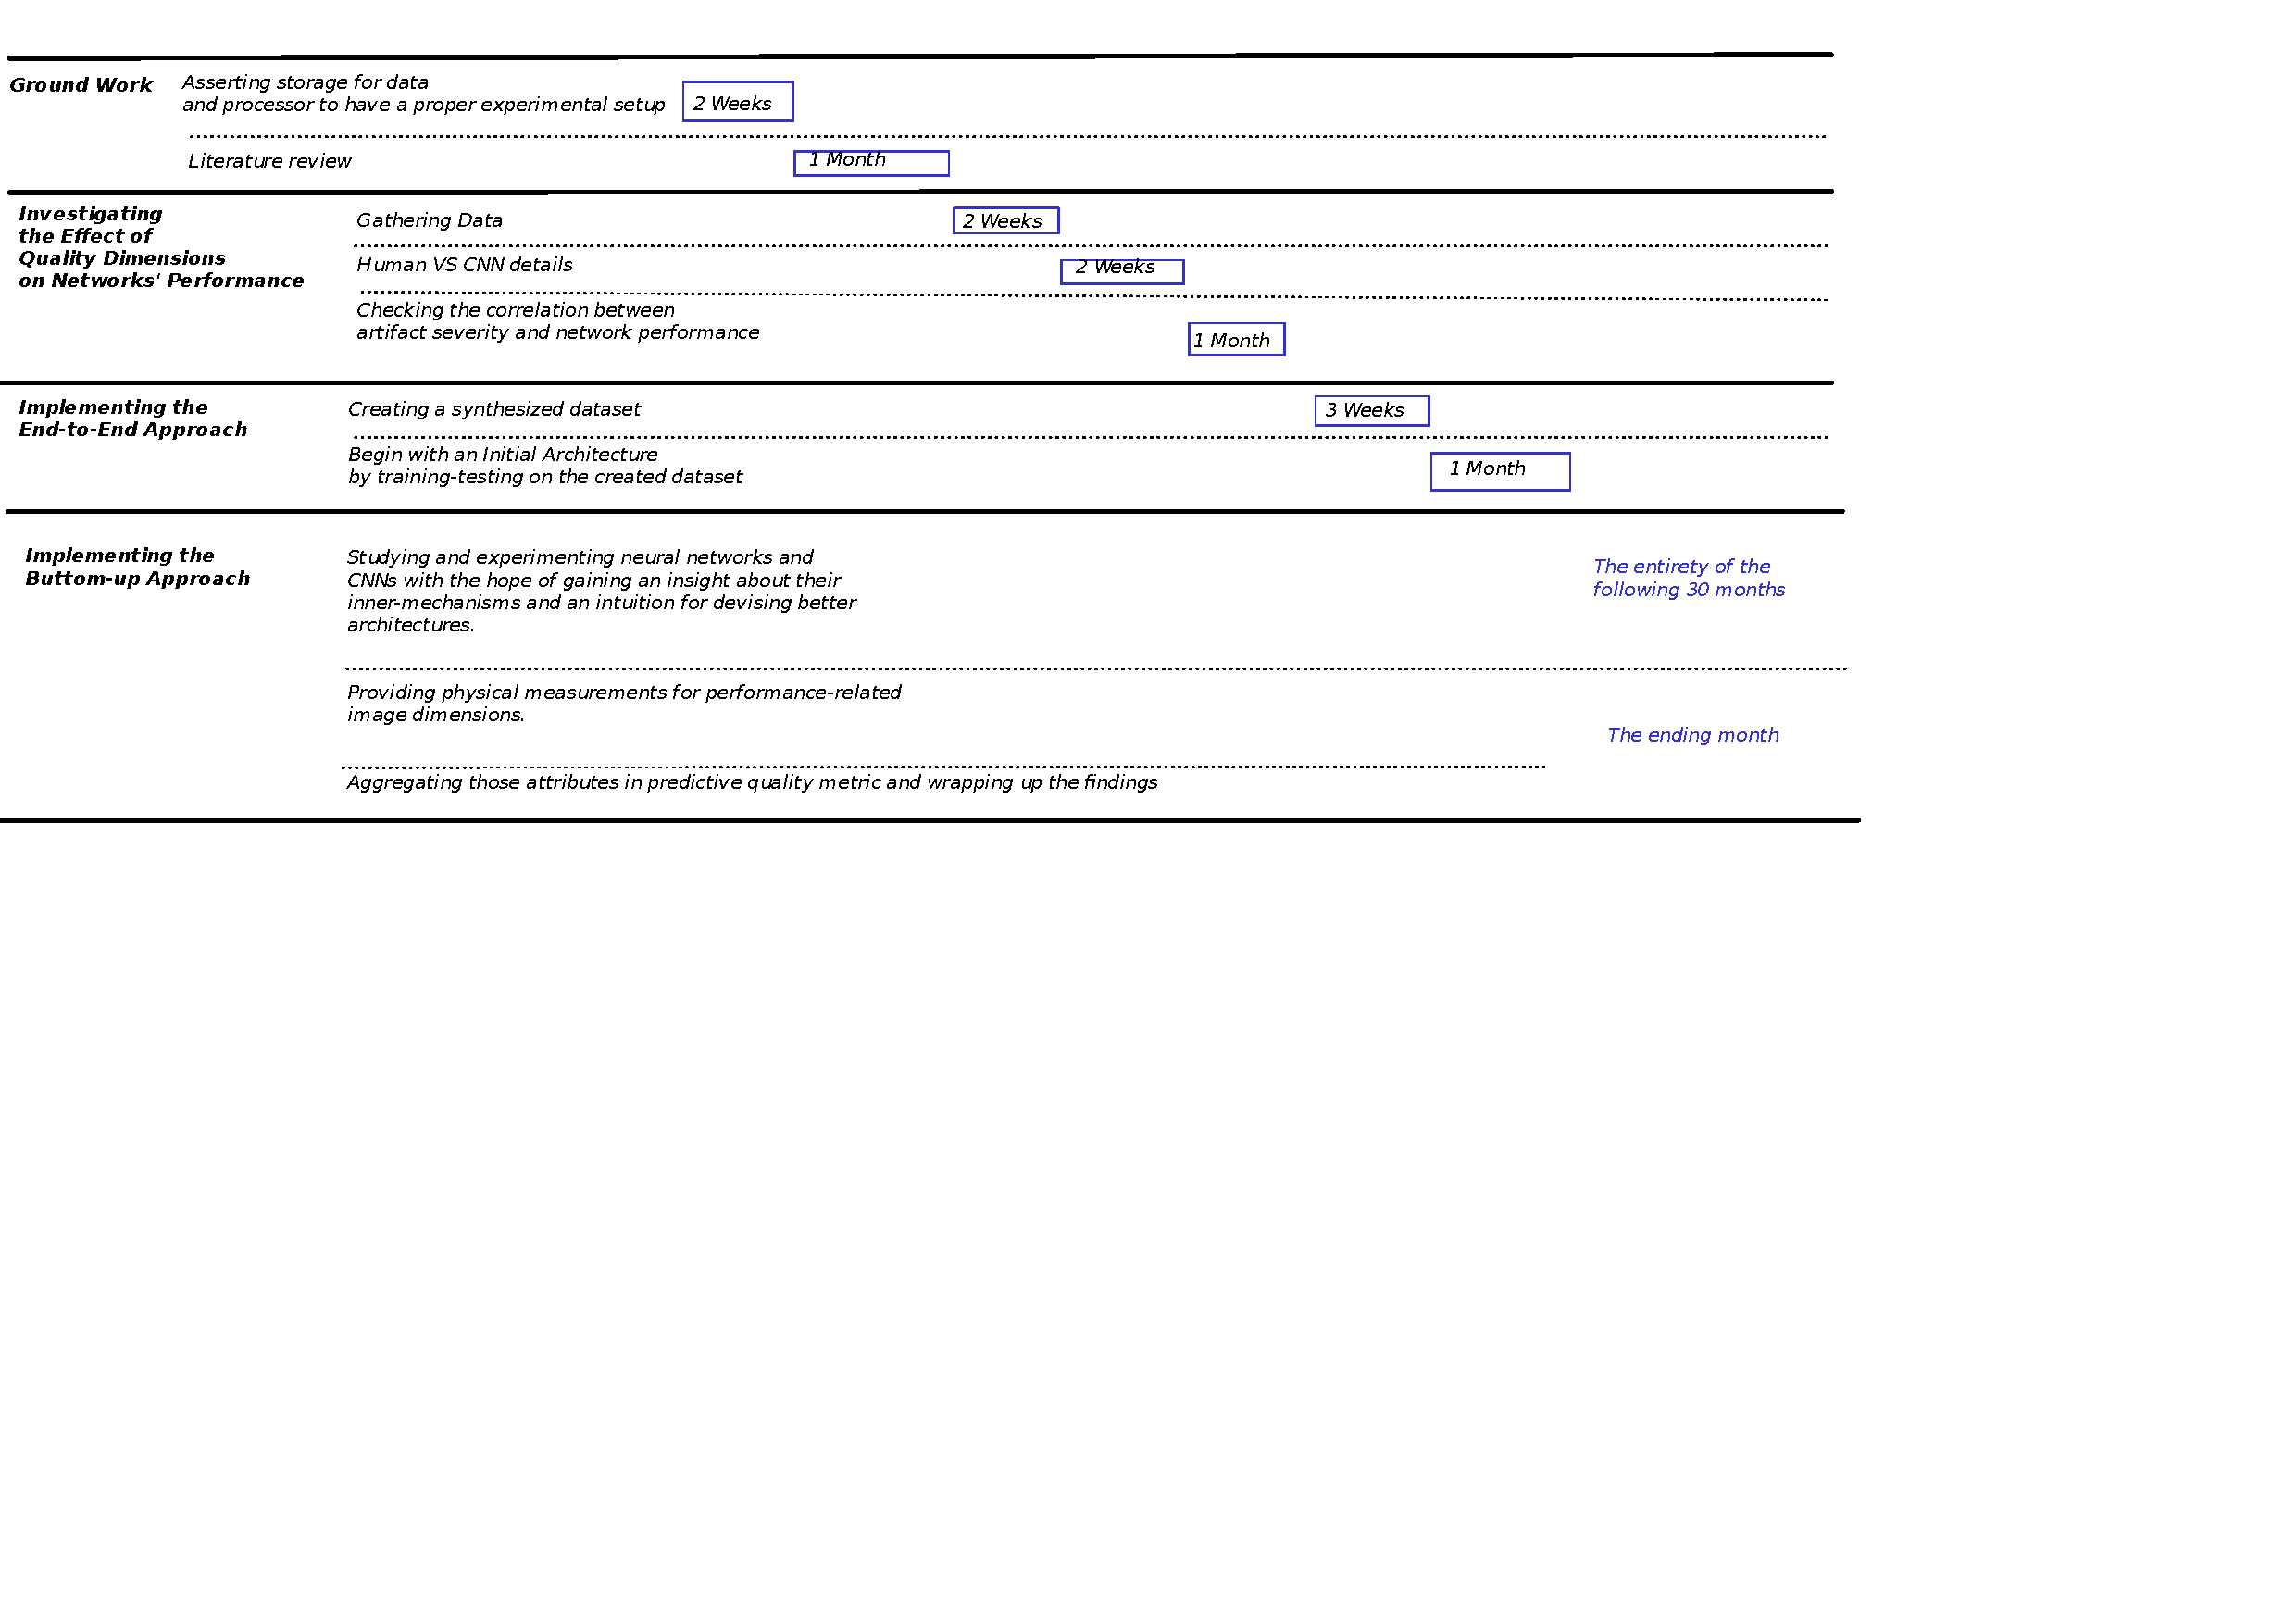
\includegraphics[trim=0 14.5cm 8cm 1cm, clip, width = 26cm]{gantt}
	\caption{Gantt chart for the proposed method}
	\label{fig:gantt}
\end{figure}
\end{landscape}
% \begin{landscape}
% \begin{table}
% 	\caption{The Gantt Chart of the Proposed Method}
% 	\label{tab:time}
% 	\scriptsize
% 	\begin{tabular}{||p{0.6pt}|p{0.6pt}||c|c|c|c|c|c|c|c|c|c|c|c|c|c|c|c|c|c|c|c|c|c|c|c|c|c|c|c|c|c|c|c|c|c|c|c||}
% 		\hline
% 		\hline
% 		\multicolumn{2}{||c||}{Task}&1&2&3&4&5&6&7&8&9&10&11&12&13&14&15&16&17&18&19&20&21&22&23&24&25&26&27&28&29&30&31&32&33&34&35&36\\
% 		\hline
% 		Ground work& Asserting storage for data and processor& \cellcolor{blue!25}&&&&&&&&&&&&&&&&&&&&&&&&&&&&&&&&&&&\\
% 	\end{tabular}
% \end{table}
% \end{landscape}
%%%%%%%%%%%%%%%%%%%%%%%%%%%%%%%%%%%%%%%%%%%%%%%%%%%%%%%%%%
%%%%%%%%%%%%%%%%%%%%%% end timing & plan %%%%%%%%%%%%%%%%
%%%%%%%%%%%%%%%%%%%%%%%%%%%%%%%%%%%%%%%%%%%%%%%%%%%%%%%%%
\bibliography{ref}
\bibliographystyle{ieeetr}
%%%%%%%%%%%%%%%%%%%%%%%%%%%%%%%%%%%%%%%%%%%%%%%%%%%%
%%%%%%%%%%%%%%% end document %%%%%%%%%%%%%%%%%%%%%%%%%
%%%%%%%%%%%%%%%%%%%%%%%%%%%%%%%%%%%%%%%%%%%%%%%%%%%%%%
\end{document}
